%added m=1 to initial conditions 
%added small description to pressure table
%removed last sentence from error calculation as it was repetitive

\documentclass{article}
\usepackage{amsmath}
\usepackage{float}
\usepackage{amssymb}
\usepackage{graphicx}
\usepackage[margin=1in]{geometry}
\usepackage{multicol,caption,listings}
\usepackage{cite}

\bibliographystyle{plain}

\begin{document}

\title{Molecular Dynamics Simulation of Argon}
\author{P. Hansler, D. Kuitenbrouwer, and A. Lovell}
\maketitle

\noindent \textbf{Abstract}  Molecular dynamics simulations are useful in a wide variety of fields from thermodynamics to biophysics to macromolecular studies.  In the 1960s, Loup Verlet performed molecular dynamics calculations for argon molecules within a Lennard-Jones potential to study their thermodynamical quantities.  In this work, we will describe the underlying structure of our own molecular dynamics simulation of argon as well as the resulting temperature, pressure, and correlation function calculations.  These will be used to investigate properties of our system and will be compared to previous results.  \\

\begin{multicols}{2}

\section{Introduction}

There is an increasing demand for knowledge of the dynamic properties of physical systems.  Where other methods such as Monte Carlo simulations are useful to find static properties of such systems, Molecular Dynamics (MD) can be used to research the dynamics of such systems.  MD is based on the equations of motion.  For this reason, MD allows tracking of the position and momentum of each particle at each moment in time.  Therefore, besides static properties, MD can be used to research how particles effect each other in multiple particle systems, which gives insight in the dynamics of such systems \cite{thijssen}.  MD is applied in many fields, for example in biological physics in the study of macromolecules \cite{deGroot} \\

In this research, the behavior of argon is simulated for different values of density and temperature.  This report focuses on how a MD simulation works.  We discuss how to translate the physical properties of multiple particle systems, such as the Lennard-Jones potential, energy conservation, and an FCC lattice to a codable form. In order to gain insight into how the material behaves for different temperatures and densities, correlation functions and pressure as function of time will be discussed. \\

This report is broken into the following sections.  In Section \ref{theory}, we will briefly discuss the theory behind the calculations in this report.  Section \ref{disc} presents the results of our calculations, including a thermostat, correlation functions for the three states of matter, and pressure calculations.  We will then give a brief conclusion in section \ref{conc}.  An appendix is found at the end of this report to discuss the method used for error analysis.  

\section{Theory}
\label{theory}

In the following subsections, we will give an overview of the concepts and equations that will be needed to build a molecular dynamics simulation of argon.

\subsection{Crystalline Array}

\begin{figure}[H]
\begin{center}

\includegraphics[width=0.65\linewidth]{plots/crystal_structure.png}
\caption{Two-dimensional unit cell of a face-central cubic (FCC) crystal.  The entire crystal can then be built up through these unit cells.}
\label{unitcell}
\end{center}
\end{figure}

The most stable and standard lattice structure of argon is face-centered cubic (FCC).  The unit cell in an FCC crystal contains four atoms in the shape of a triangular pyramid, Figure \ref{unitcell}.  In the FCC lattice, the sheets of atoms stack on top of each other in such a way that every other layer is off-set by half of an atomic radius, Figure \ref{fcc}, left.  (This is in contrast to a HCP - hexagonal close packed - lattice where every other sheet of atoms lines up, Figure \ref{fcc}, right.)  \cite{crystal}  We use the FCC configuration for the initial conditions of our simulation because the equilibrium state of argon is an FCC lattice.  

\begin{figure}[H]
\begin{center}
\begin{tabular}{ c c }
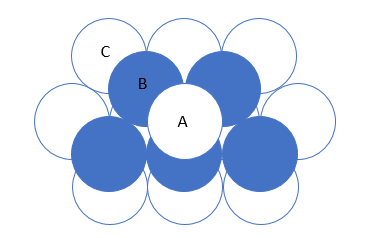
\includegraphics[width=0.45\linewidth]{plots/fcc_crystal.png} & 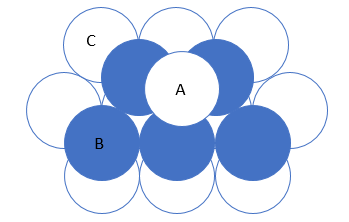
\includegraphics[width=0.45\linewidth]{plots/hcp_crystal.png}
\end{tabular}
\caption{Left, structure of an FCC crystal.  Right, structure of an HCP crystal.  In the FCC crystal, layers A and C are off-set by the radius of one of the particles in the lattice (represented by the blue and white circles).  A fourth layer on top of A would line up again with layer C.  In contrast, in the HPC structure, layers A and C directly overlap.}
\label{fcc}
\end{center}
\end{figure}

\subsection{Interaction}

To describe the interaction between each of the argon atoms, we use the Lennard-Jones potential \cite{verlet}, which accounts for the short-range repulsive force between the two atoms due to Coulomb repulsion and the longer-range attractive forces from dipole-dipole and dipole-induced dipole forces.  The form of the potential is as follows:

\begin{equation}
V_{LJ}(r) = 4 \epsilon \left [ \left (\frac{\sigma}{r} \right )^{12} - \left (\frac{\sigma}{r} \right )^{6} \right ]
\label{LJpot}
\end{equation}

\noindent where $r$ is the distance between the two atoms, $\epsilon$ gives the depth of the potential well, and $\sigma = 2R $ where $R$ is the internuclear distance between the two atoms - $\sigma$ measures the distance at which the potential between the two particles is zero.  An example of the Lennard-Jones potential can be found in Figure \ref{VLJfig}. \\

When the two atoms are far enough apart, they can be viewed as non-interacting.  For this reason, we can introduced a cut-off radius, $r_c$, beyond which the potential between two particles is taken to be zero.  Thus, we use the interaction 

\begin{equation}
V_{LJ} (r) = \begin{cases}
4 \epsilon \left [ \left (\frac{\sigma}{r} \right )^{12} - \left (\frac{\sigma}{r} \right )^{6} \right ] & r \le r_c \\
0 & r > r_c
\end{cases}
\label{cutoff}
\end{equation}

From (1), we immediately know the form of the force between the two atoms as well.  The force is radial, acting to bring the atoms closer together if $r > r_{\mathrm{min}}$ and repelling them if $r < r_{\mathrm{min}}$, where $r_{\mathrm{min}}$ is where the potential well has its minimum (approximately 1.1 fm in Figure \ref{VLJfig}).  For our purposes, it it convenient to write the forces in terms of their Cartesian coordinates.  

\begin{equation}
\begin{split}
F_x = 24\epsilon x \left [ \frac{2 \sigma ^{12}}{r^{14}} - \frac{\sigma ^{6}}{r^8} \right ] \\
F_y = 24 \epsilon y \left [ \frac{2 \sigma ^{12}}{r^{14}} - \frac{\sigma ^{6}}{r^8} \right ] \\
F_z = 24 \epsilon z \left [ \frac{2 \sigma ^{12}}{r^{14}} - \frac{\sigma ^{6}}{r^8} \right ] \\
\end{split}
\end{equation}

\noindent From the force between each pair of particles, the momenta and positions can be calculated, leading to the dynamics of the system.  This also allows calculation of thermodynamical quantities, such as temperature, energy, pressure, chemical potential, and correlation function.\\

\begin{figure}[H]
\begin{center}
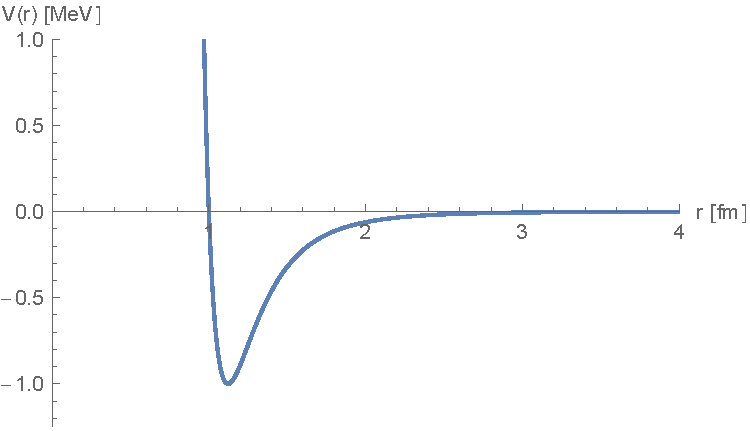
\includegraphics[width=\linewidth]{plots/VLJ.pdf}
\caption{The shape of the Lennard-Jones potential.  Here, $\sigma=1$ fm (the distance where the potential crosses the r-axis) and $\epsilon =1$ MeV (the maximum depth of the interaction).}
\label{VLJfig}
\end{center}
\end{figure}

\subsection{Velocity Verlet Method}

The method chosen for the position and momentum calculations is the Verlet method.  While both can be calculated from the introductory physics equations,

\begin{equation}
\label{momeqn}
p_{i+1}=p_i + F \Delta t
\end{equation}

\noindent and

\begin{equation}
\label{poseqn}
x_{i+1} = x_i + \frac{p_i}{m} + \frac{1}{2}\frac{F(\Delta t)^2}{m}
\end{equation}

\noindent this can lead to numerical inaccuracies in the position calculation because of the dependence on the square of the time step and both the previous force and momentum.  The advantages of using the Verlet method are its accuracy, stability and its tendency to traject the same path in phase space within numerical precision.  In our simulation we will need the momenta and positions at every time step to calculate parameters such as energy.  A variety of the Verlet method which accomplishes this is known as the Verlet velocity scheme \cite{verlet}.

% link: http://www.physics.udel.edu/~bnikolic/teaching/phys660/numerical_ode/node5.html

\begin{equation}
\label{verletvscheme}
\begin{split}
p_{i+\frac{1}{2}}=p_i + \frac{F_i}{2} \Delta t \\
r_{i+1}=r_i+\frac{p_{i+\frac{1}{2}}}{m} \Delta t \\
F_{i+1}=-\frac{1}{m} \frac{\partial V_{LJ}(r_i)}{\partial r} \\
p_{i+1} = p_{i+\frac{1}{2}} + \frac{F_{i+1}}{2} \Delta t \\
\end{split}
\end{equation}

\subsection{Thermodynamics}
\label{thermo}

Along with updating the position an momentum of each particle to see how the system equilibrates, there are also several thermodynamic quantities that we can calculate in order to learn more about the system we have created.  Before calculating any quantities, we want to model our system as being in contact with a thermostat to keep it at a constant temperature.  We do this by renormalizing the velocity in the following manner.  \\

Through the Equipartition Theorem, the average velocity and temperature of a system are related by

\begin{equation}
\label{vir}
\frac{1}{2}m \langle v^2 \rangle = \frac{3}{2} k_B T
\end{equation}

\noindent where $m$ is the mass of the system, $\langle v^2 \rangle$ is the time average of the square of the velocity, $k_B$ is Boltzmann's constant (equal to one in a system where we take temperature and energy to have the same unit), and $T$ is the temperature of the system.  Therefore, to enforce a target temperature, $T_o$ in our system, the system must have a certain average velocity, $\langle v^2 \rangle _o$ given by

\begin{equation}
\label{virknot}
\frac{1}{2}m \langle v^2 \rangle _o = \frac{3}{2} k_B T_o
\end{equation}

Dividing (\ref{vir}) by (\ref{virknot}) and taking the square root of each side, we have

\begin{equation}
\sqrt{\frac{\langle v^2 \rangle}{\langle v^2 \rangle _o}} = \left ( \frac{T}{T_o} \right ) ^{1/2}
\end{equation}

\noindent Thus we can renormalize each velocity with 

\begin{equation}
v = \lambda v_o
\end{equation}

\noindent where $\lambda = (T/T_o)^{1/2}$ to ensure a constant temperature.  \\

To calculate the temperature of a system, we again make use of the Equipartition Theorem (\ref{vir}), taking into account the number of particles in the system in the following way

\begin{equation}
\frac{1}{2}N m \langle v^2 \rangle = \frac{3}{2} (N-1) k_B T
\end{equation}

\noindent The temperature of the system is then found by rearranging the above equation

\begin{equation}
T = \frac{Nm \langle v^2 \rangle}{3(N-1)k_B}
\end{equation}

\noindent which can easily be written in terms of the total kinetic energy of the system $E_{kin} = \frac{N}{2} \langle v^2 \rangle $.  \\

Once the system is at a constant temperature, we can calculate the correlation function.  The correlation function measures the amount of disorder in a system, and therefore gives a distinct shape based on the state of matter - solid, liquid or gas.  To calculate the correlation function, $g(r)$, we count the number of particles inside a spherical shell of $r + \delta r$ and normalize by the volume of that shell.  Taking $\delta r$ to be much smaller than $r$, we can approximate the volume of each shell by

\begin{equation}
\begin{split}
\Delta V & = \frac{4}{3} \pi (r+\delta r)^3 - \frac{4}{3} \pi r^3 \\
& = \frac{4}{3} \pi \left [ r^3 \left (1+\frac{\delta r}{r} \right )^3 - r^3 \right ] \\
& = \frac{4}{3} \pi \left [ r^3 \left ( 1 + 3\frac{\delta r}{r} + \mathcal{O} (\delta r ^2) \right ) - r^3 \right ] \\
& = 4 \pi r^2 \delta r
\end{split}
\end{equation}

\noindent where the third line uses the Taylor approximation of $(1+z)^n = 1 + nz+ ...$  Taking the total volume, the number of particles, and double counting into account, we arrive at the correlation function (\ref{corfunceq}). 

\begin{equation}
g(r) = \frac{2VN_r}{N(N-1)4 \pi r^2 \delta r}
\label{corfunceq}
\end{equation}

\noindent where $N_r$ is the number of particles found in the shell $r + \delta r$.  \\

In order to obtain a time averaged correlation function, the correlation function is calculated for each time step after the renormalization has been switched off. Especially for higher temperatures, the correlation function fluctuates a bit for distances greater than $2\AA$. Therefore it makes sense to take a time average, so that an accidental fluctuation would not be evaluated as an actual correlation. In the code, this is taken into account by dividing by the number of time steps. \\

The correlation function has distinct shapes for each state of matter.  Solids are classified by period spikes which indicates a lattice of particles.  Liquids look like a decaying periodic function.  Last, gases show an exponential-like decay in their correlation function.  These are the characteristics we will be looking to explore in our calculations. \\

%\noindent Another physical quantity that can be calculated is the pressure. The pressure can be calculated by making use of the following formula:

%\begin{equation}
%  = \frac{NK_{B}T}{V} + \frac{1}{3V}\avg{\sum\limits_{i}^N %R_{ij}\frac{\partial u(r)}{\partial R_{ij}}} - \frac{2$\pi%$N^2}{3V^2}\int_R_{c}^\inf\! R^3 \frac{\partial u(r)}{\partial R}g(r)dR
%\end{equation}

Another physical quantity that can be calculated is the pressure of the system.  With a constant temperature, the pressure of a system can be found using the Virial Theorem.  Using Hamilton's equations

\begin{equation}
\begin{split}
\dot{\textbf{r}}_a = \textbf{v}_a \\
\dot{\textbf{p}}_a = \textbf{F}_a 
\end{split}
\end{equation}

\noindent and taking the time average of $\sum \limits _a (\textbf{r}_a \cdot \textbf{p}_a)$, we have

\begin{equation}
\begin{split}
\overline{\frac{d}{dt} \sum \limits _a \textbf{r}_a \cdot \textbf{p}_a} & = \overline{\sum \limits _a \textbf{v}_a \cdot \textbf{p}_a + \textbf{r}_a \cdot \textbf{F}_a} \\
& = 0
\end{split}
\end{equation}

\noindent  For non-relativistic particles 

\begin{equation}
K = \sum \limits _a \frac{\textbf{p}_{a}^2}{2m_a}
\end{equation}

\noindent and 

\begin{equation}
\begin{split}
\overline{\sum \limits _a \textbf{v}_a \cdot \textbf{p}_a} & = 2\bar{K} \\
& = - \overline{\sum \limits _a \textbf{r}_a \cdot \textbf{F}_a}
\end{split}
\end{equation}

\noindent This gives the Virial term between two particles.  We can add this term to our expected energy-pressure relation for non-interacting particles, $\bar{K}=\frac{3}{2}PV$, to find the total average kinetic energy of a system of interacting particles:  

\begin{equation}
\bar{K} = \frac{3}{2} PV - \frac{1}{2} \overline{\sum \limits _{a \ne b} r_{ab} F(r_{ab})}
\end{equation}

\noindent from here, straight-forward algebraic manipulations give the pressure.

\begin{equation}
P = \frac{2}{3V} \left [ \bar{K} + \frac{1}{2} \overline{\sum \limits _{a\ne b} r_{ab} F(r_{ab})} \right ]
\label{hampres}
\end{equation}

\noindent Here, $r_{ab} = |\textbf{r}_a - \textbf{r}_b|$, the distance between any pair of particles. \\

The second term of the right hand side of (\ref{hampres}) consist of the forces between each pair of particles (the negative of the gradient of the Lennard-Jones potential).  This is the same force that is used in the Verlet Algorithm to update the momenta.  In order to save computation time, these same forces could be used here.  However, for reasons of calculation speed, the forces were only calculated between particles that were within a certain range $r_c$ (recall equation (\ref{cutoff})). For this reason we need to split up the previously mentioned term in equation (\ref{hampres}) in a region where $0 < r < r_c $ and a region where $ r_c < r < \infty $. This results in the following equation.

\begin{equation}
\begin{split}
P = \frac{N k_B T}{V} - \frac{1}{3 V} \langle \sum\limits_{i=1}^N \sum\limits_{j>i}^N r_{ij} \frac{\partial V_{LJ}(r)}{\partial r}\rangle_{r < r_c} \\
- \frac{2 \pi N^2}{3 V^2} \int_{r_c}^\infty r^3 \frac{\partial V_{LJ}(r)}{\partial r} g(r) dr
\label{prescomp}
\end{split}
\end{equation}

\noindent The last term in this equation can be calculated once numerically since for $R>R_c$, $g(R) = 1$. For the values of $\epsilon$ and $\sigma$ in the Lennard-Jones potential mentioned in Section \ref{IC}, the value for the integral is $0.9756$.

\section{Discussion}
\label{disc}

In the following subsections, we present the results of our simulation.  First, we describe the initial conditions under which our simulation was performed and show that our system conserves energy.  Next, we argue that our system is modeled to be in contact with a thermostat of variable temperature.  Finally, we present the correlation functions and pressures for each of our simulations of a solid, liquid, and gas.

\subsection{Initial Conditions}
\label{IC}

We started with our system in a face-centered cubic crystalline configuration (recall Figure \ref{fcc}).  Our simulation modeled 864 argon atoms with a unit cell length dependent on the density of the system.  The initial positions were determined by the crystalline structure of an FCC lattice, and the initial velocities were randomly picked from a Maxwell-Boltzmann distribution centered around and average velocity of zero and standard deviation of $\sqrt{T}$, where $T$ denotes the temperature of the system.  The boundary conditions of our system were periodic; every time a particle crossed outside of the box by a distance $b$, is was taken to be at a position $L-b$ inside of the box (where the length of the box is $L$).  This simulates a particle moving continuously, regardless of box size.  The cut-off distance where the particles were taken to be non-interacting was $r_c = 3.2$ $\AA$, and the time step for the Verlet method was $\Delta t = 0.004$ s.  Each simulation was run for 10,000 time steps, which was found to be long enough to bring our system to equilibrium.  As mentioned previously, we will take $\sigma=\epsilon=m=k_B=1$, which also gives us a system where temperature and energy are measured in the same units.  

\subsection{Energy Conservation}

To test that our simulation was working correctly, we first calculated the total energy of the system, which should be constant over the length of the simulation.  One such example is found in Figure \ref{engcons}.  This exercise helped us find a reasonable time step and range of temperatures.  With too large of a time step, the particles could be moved into the highly repulsive region of another's potential, which is clearly unphysical. The particle is then essentially moving too fast to respond to the potentials of the other particles around it. As a result, when the particle is located in this highly repulsive region, the particles will be bounced off with very high velocities which makes the energy blow up. On the other hand, a time step that is too small can cause a time-intensive computation and provide a level of detail that is not beneficial to this type of simulation. \\

In Figure \ref{engcons}, it can be seen that when the thermostat, which is discussed in the next section, is switched off, the total energy remains constant (after 2,000 time steps).  From Figure \ref{engcons}, the total energy, which is the sum of the kinetic and potential energies, is negative.  This is due to the large amount of negative potential energy, as can be derived from the potential in equation (\ref{LJpot}).   We can also see that both the kinetic and the potential energies fluctuate, but these fluctuations balance out in the total energy. These fluctuations have influence on the pressure and temperature, as will be discussed later.\\

To ensure that energy is conserved, we must also keep the temperature in a reasonable range.  Because we have taken $k_B =1$, energy and temperature are measured with the same units.  If we take this to be electron volts, the conversion factor is $1 $ eV $\approx 11600$ K.  Thus, as temperature increases, we quickly enter a realm where the particles are traveling at relativistic speeds.  Our simulation is purely classical and thus not equipped to accurately calculate relativistic simulations.

\begin{figure}[H]
\begin{center}
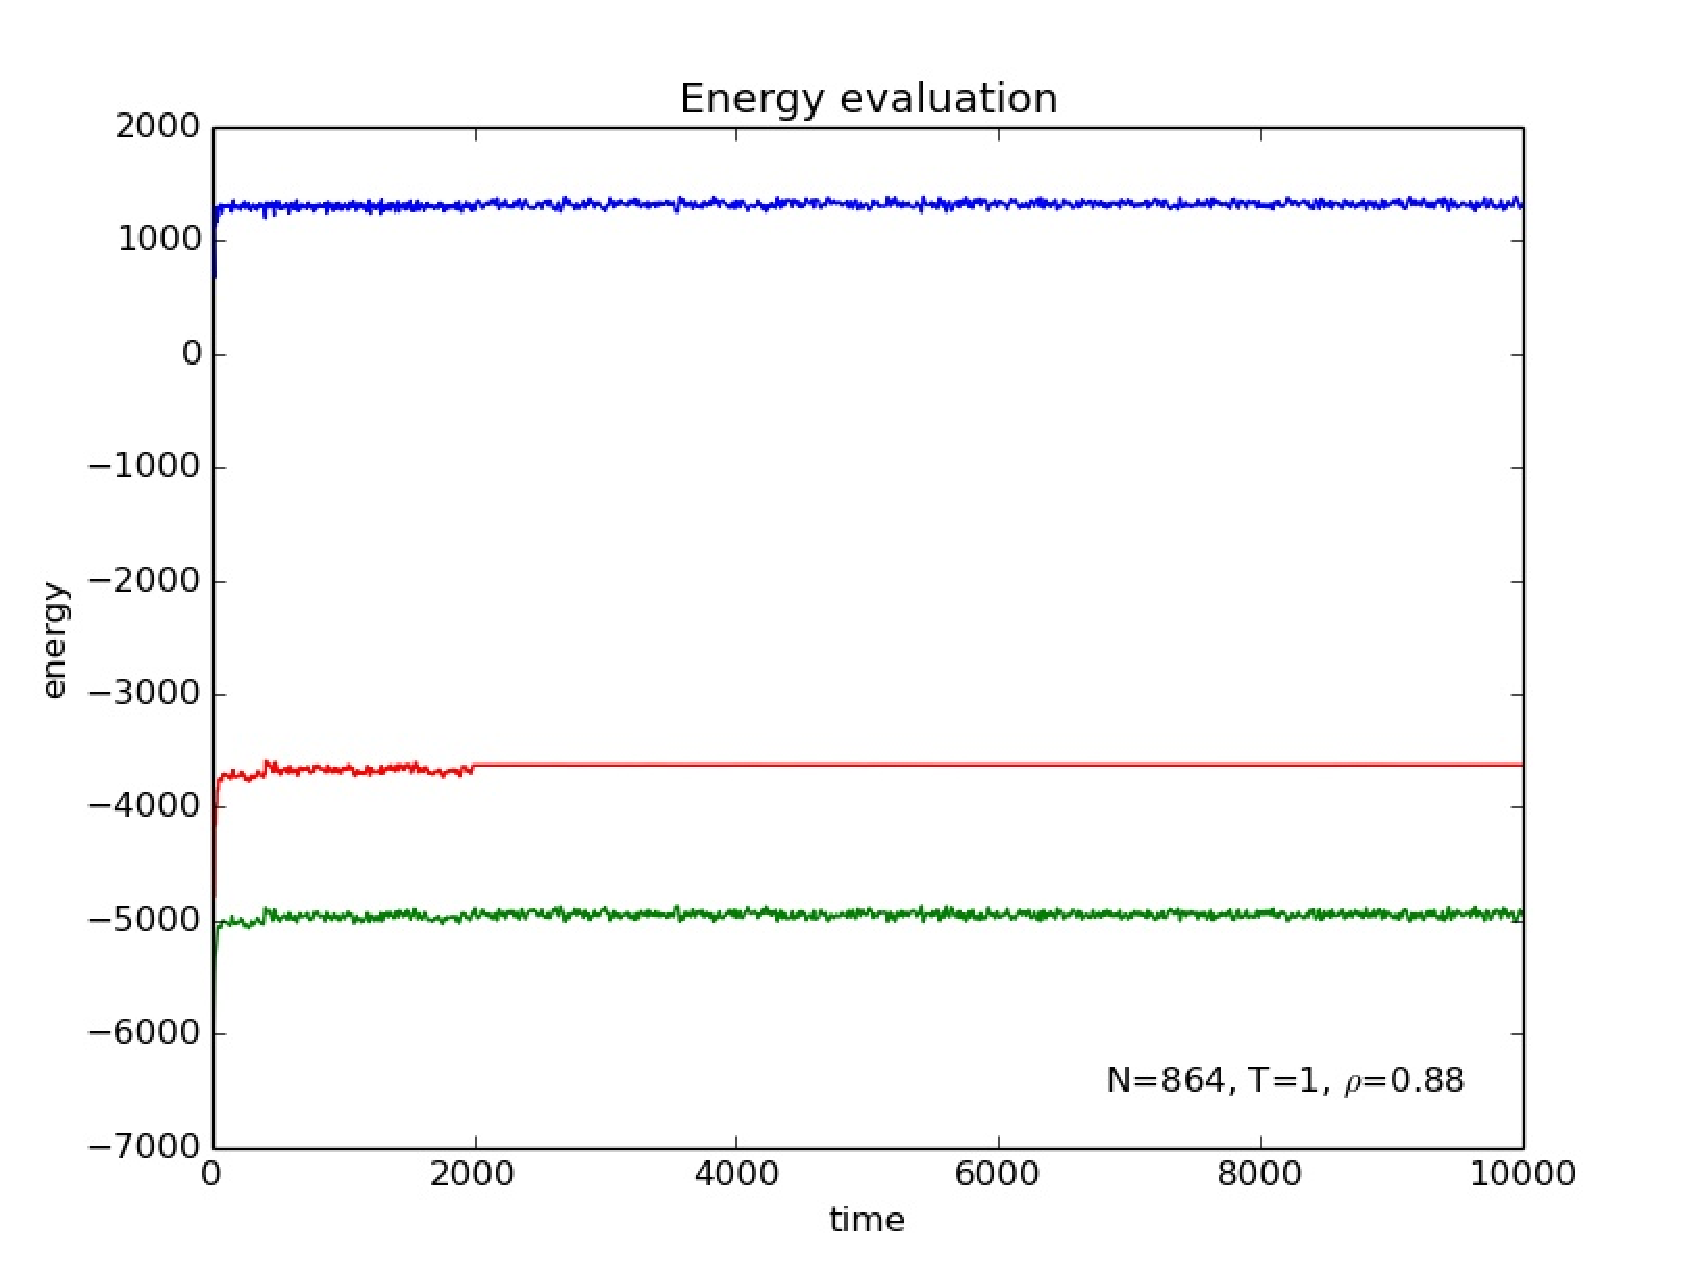
\includegraphics[width=\linewidth]{plots/energyT1rho088N864lpnum1000.pdf}
\caption{Energy as a function of time step for 864 particles, with $T=1$ eV and $\rho = 0.88$ $\AA ^{-3}$.  The blue line is the kinetic energy, the red line is the total energy and the green line is potential energy.}
\label{engcons}
\end{center}
\end{figure}

\subsection{Thermostat}

Using the renormalization method explained in Section \ref{thermo}, we were able to bring our system to any given target temperature (non-relativistic) from any starting temperature.  Some of these target temperatures and the temperature that the system actually reached together with their standard deviations are given in Table 1. \\

The temperature is directly related to the kinetic energy, as earlier discussed. Since the kinetic energy fluctuates, we find fluctuations in the temperature as well. Though, due to the fact that the standard deviation of the temperature is about a factor $100$ smaller than the actual temperature, we can conclude that fluctuations in temperature are small. \\

In Figure \ref{engrenorm}, one can see how the renormalization influences both the kinetic and the total energy. Since the initial temperature was lower than the target temperature, it is clear that the total energy goes up stepwise. Also, one can see that there are some sudden increases in the kinetic energy. These occur due to the fact that for each renormalization the velocity of the particles is suddenly increased. 

\begin{figure}[H]
\begin{center}
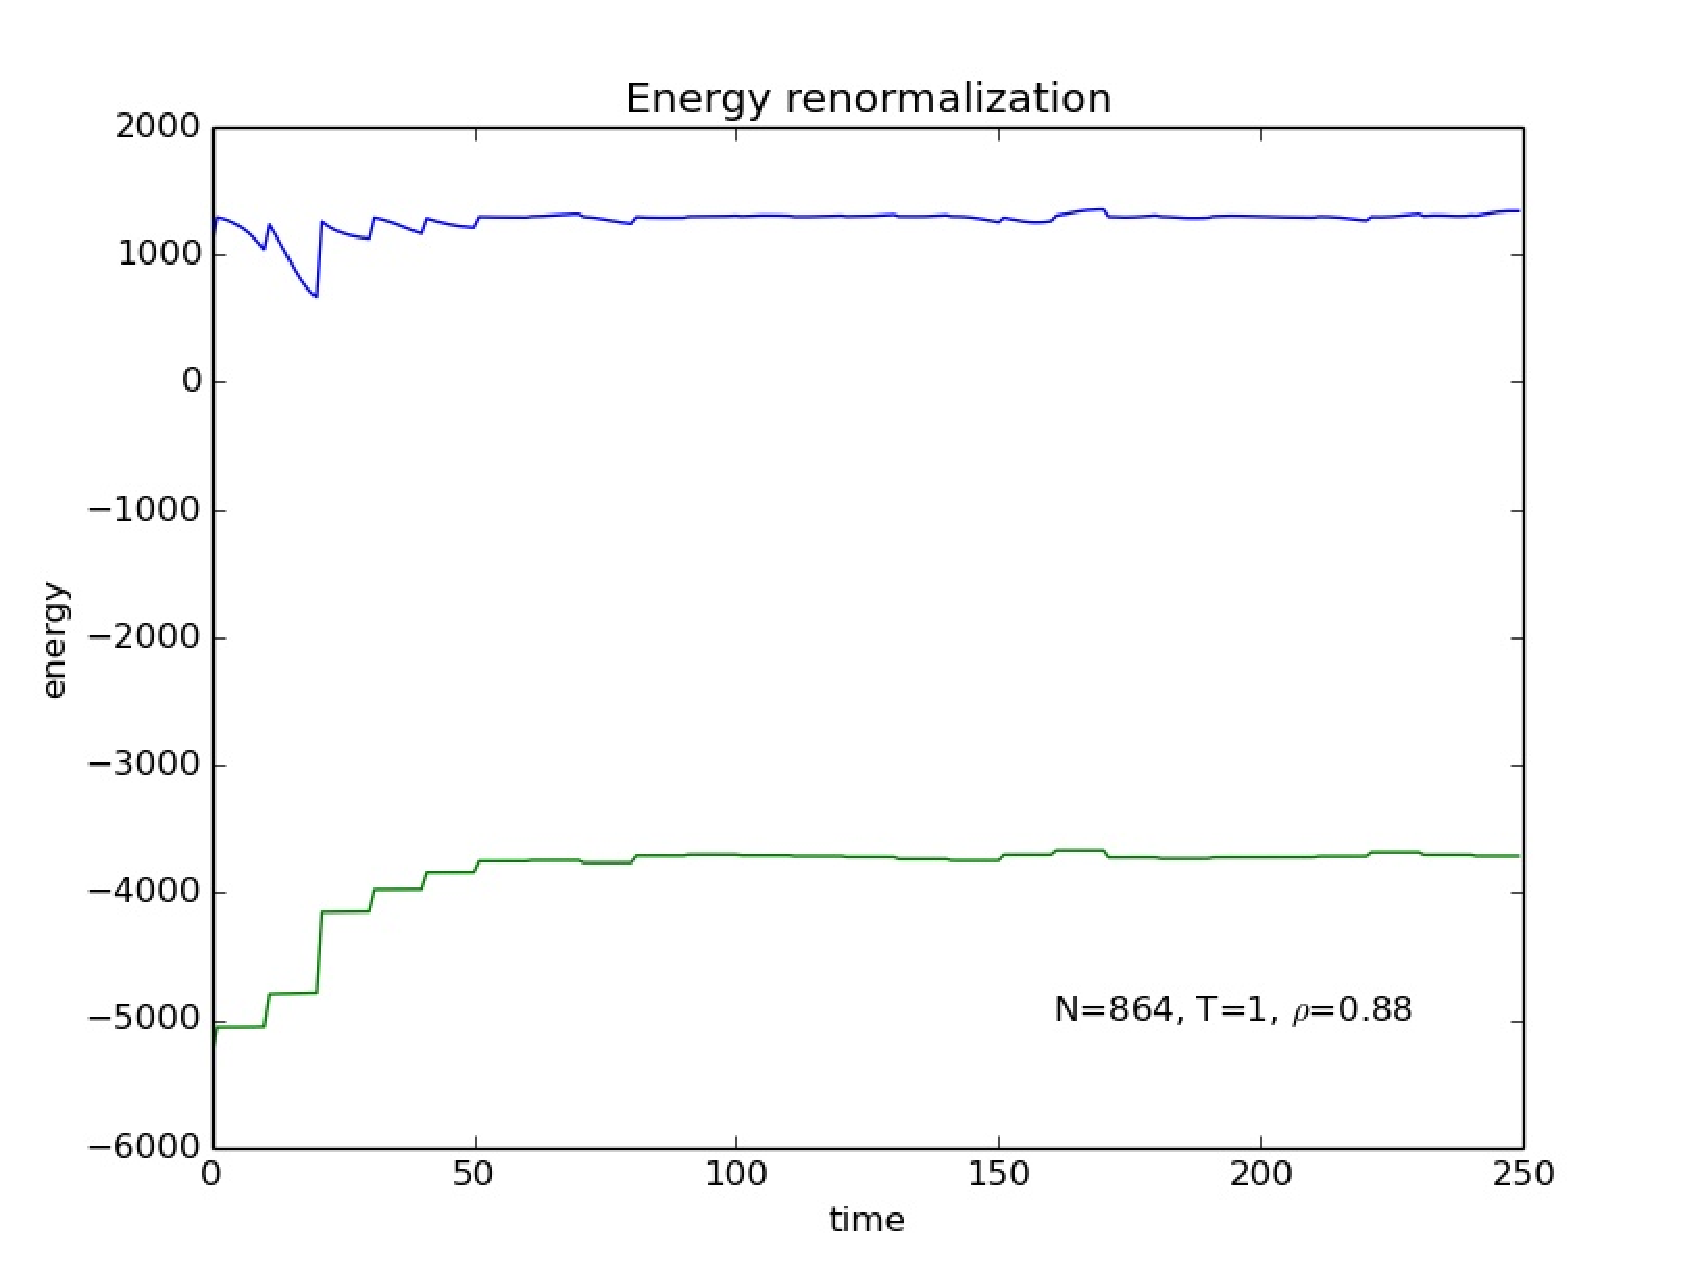
\includegraphics[width=\linewidth]{plots/renormalizationshorttimerange.pdf}
\caption{Plot of the renormalized energy (calculated with the renormalized velocity) over 250 time steps, with a renormalization every 10 steps.  The green line is the total energy and the blue line is the kinetic energy.}
\label{engrenorm}
\end{center}
\end{figure}

\begin{table*}
\begin{center}
\begin{tabular}{| c | c | c | c |}
\hline $T_{targ}$ [eV] & $T$ [eV] & $\sigma_T$ [eV] & $\sigma_T/\sqrt{N}$ [eV] \\ \hline
 0.5 & 0.499830 & 0.009934 & 0.000111 \\ \hline
1.0 & 1.015010 & 0.018228 & 0.000203  \\ \hline
3.0 & 2.975473 & 0.032667 & 0.000365 \\ \hline
\end{tabular}
\label{temptable}
\caption{Calculated temperatures, $T$, for each target temperature, $T_{targ}$, their standard deviations $\sigma _T$, and the error on calculated temperature, $\sigma _T/\sqrt{N}$, given as $T \pm \sigma_T /\sqrt{N}$, used throughout the remainder of the calculations.}
\end{center}
\end{table*}


\subsection{Correlation Function}

\begin{figure}[H]
\begin{center}
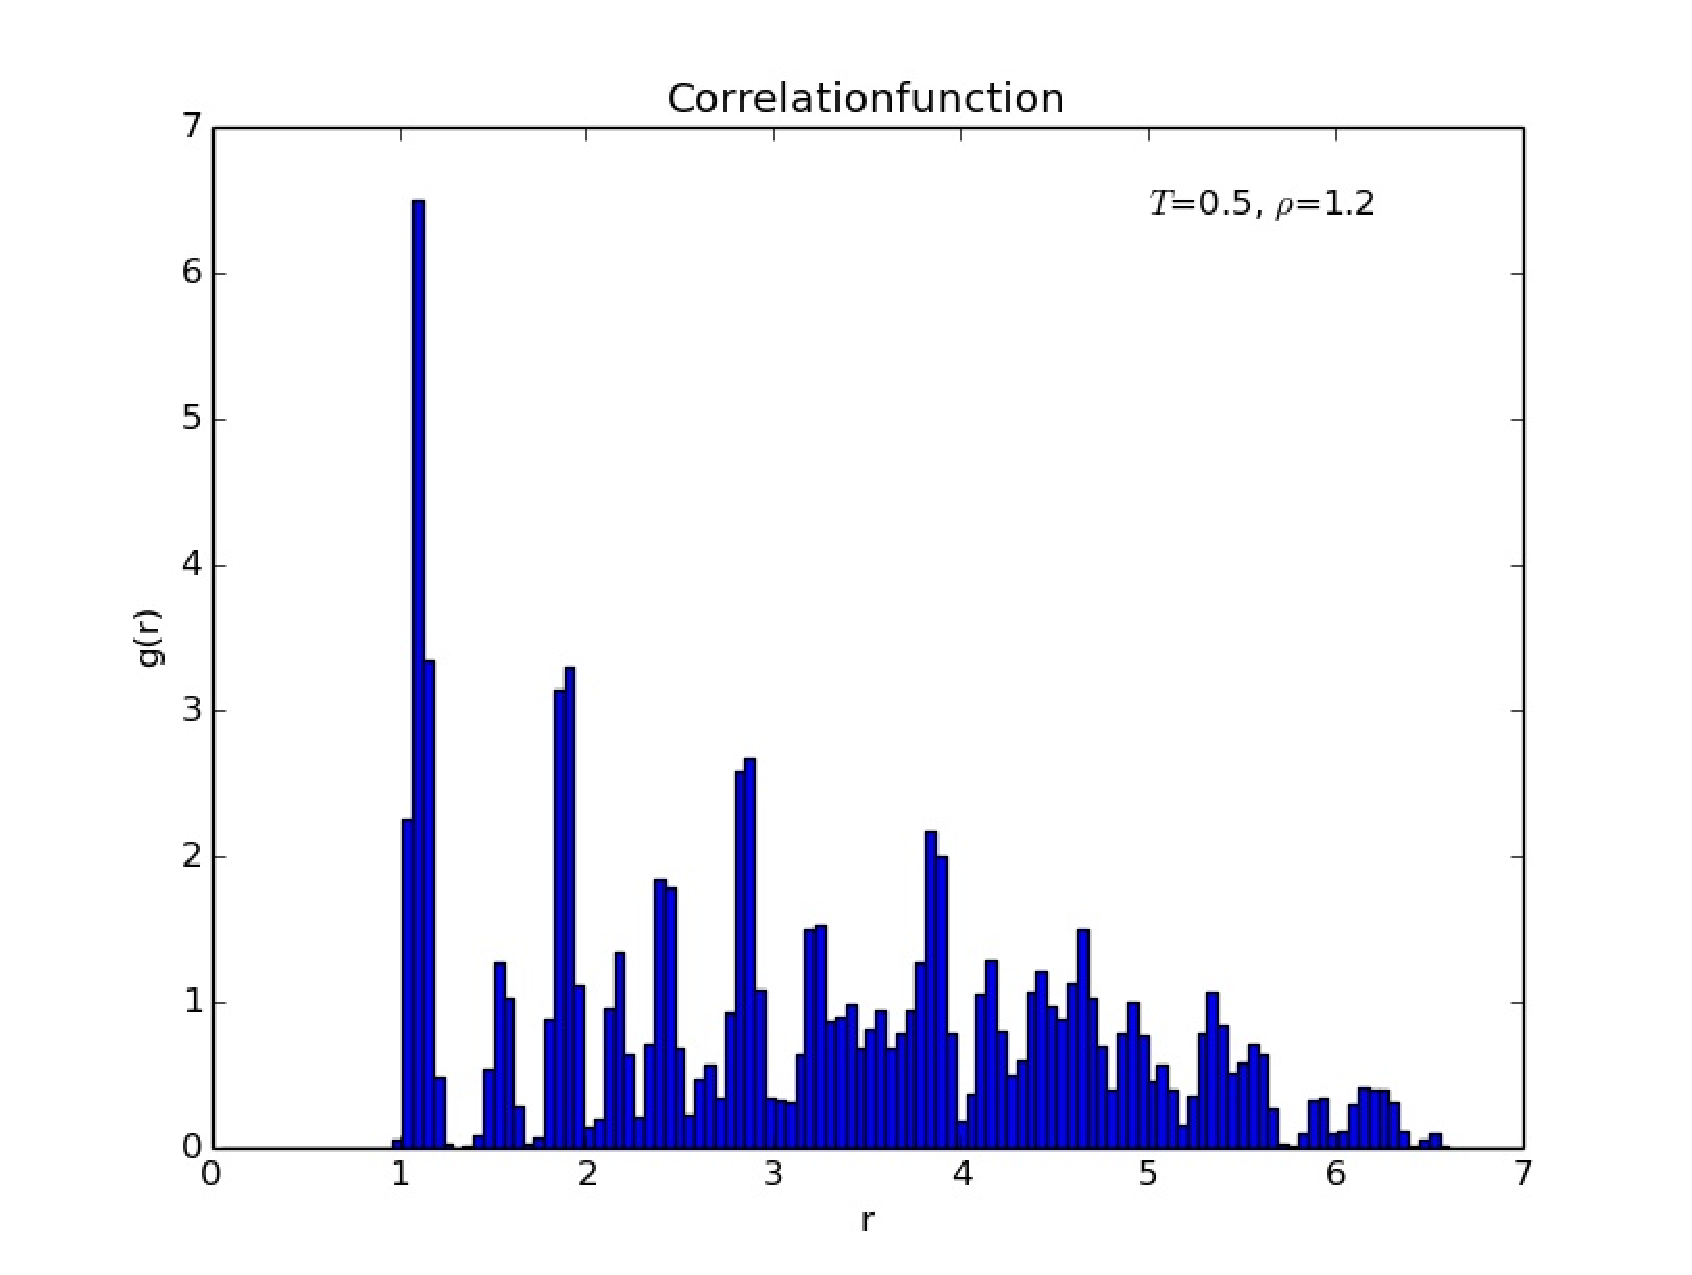
\includegraphics[width=\linewidth]{plots/correlationfunctionT05rho12x.pdf}
\caption{Correlation function for a solid at $T=0.5$ eV and $\rho=1.2$ $\AA ^{-3}$.  This periodic structure is what we would expect from a solid.}
\label{corsolid}
\end{center}
\end{figure}

Once a thermostat was established, correlation functions could be calculated.  As mentioned earlier, these give us a sense of what state of matter our system is in for different combinations of temperatures and densities.  At a low temperature and relatively high density, we confirmed that our system had properties of a solid (Figure \ref{corsolid}), at intermediate temperatures and densities, our system had properties of a liquid (Figure \ref{corliquid}), and at a high temperature and low density, our system displayed properties of a gas (Figure \ref{corgas}).  


\begin{figure}[H]
\begin{center}
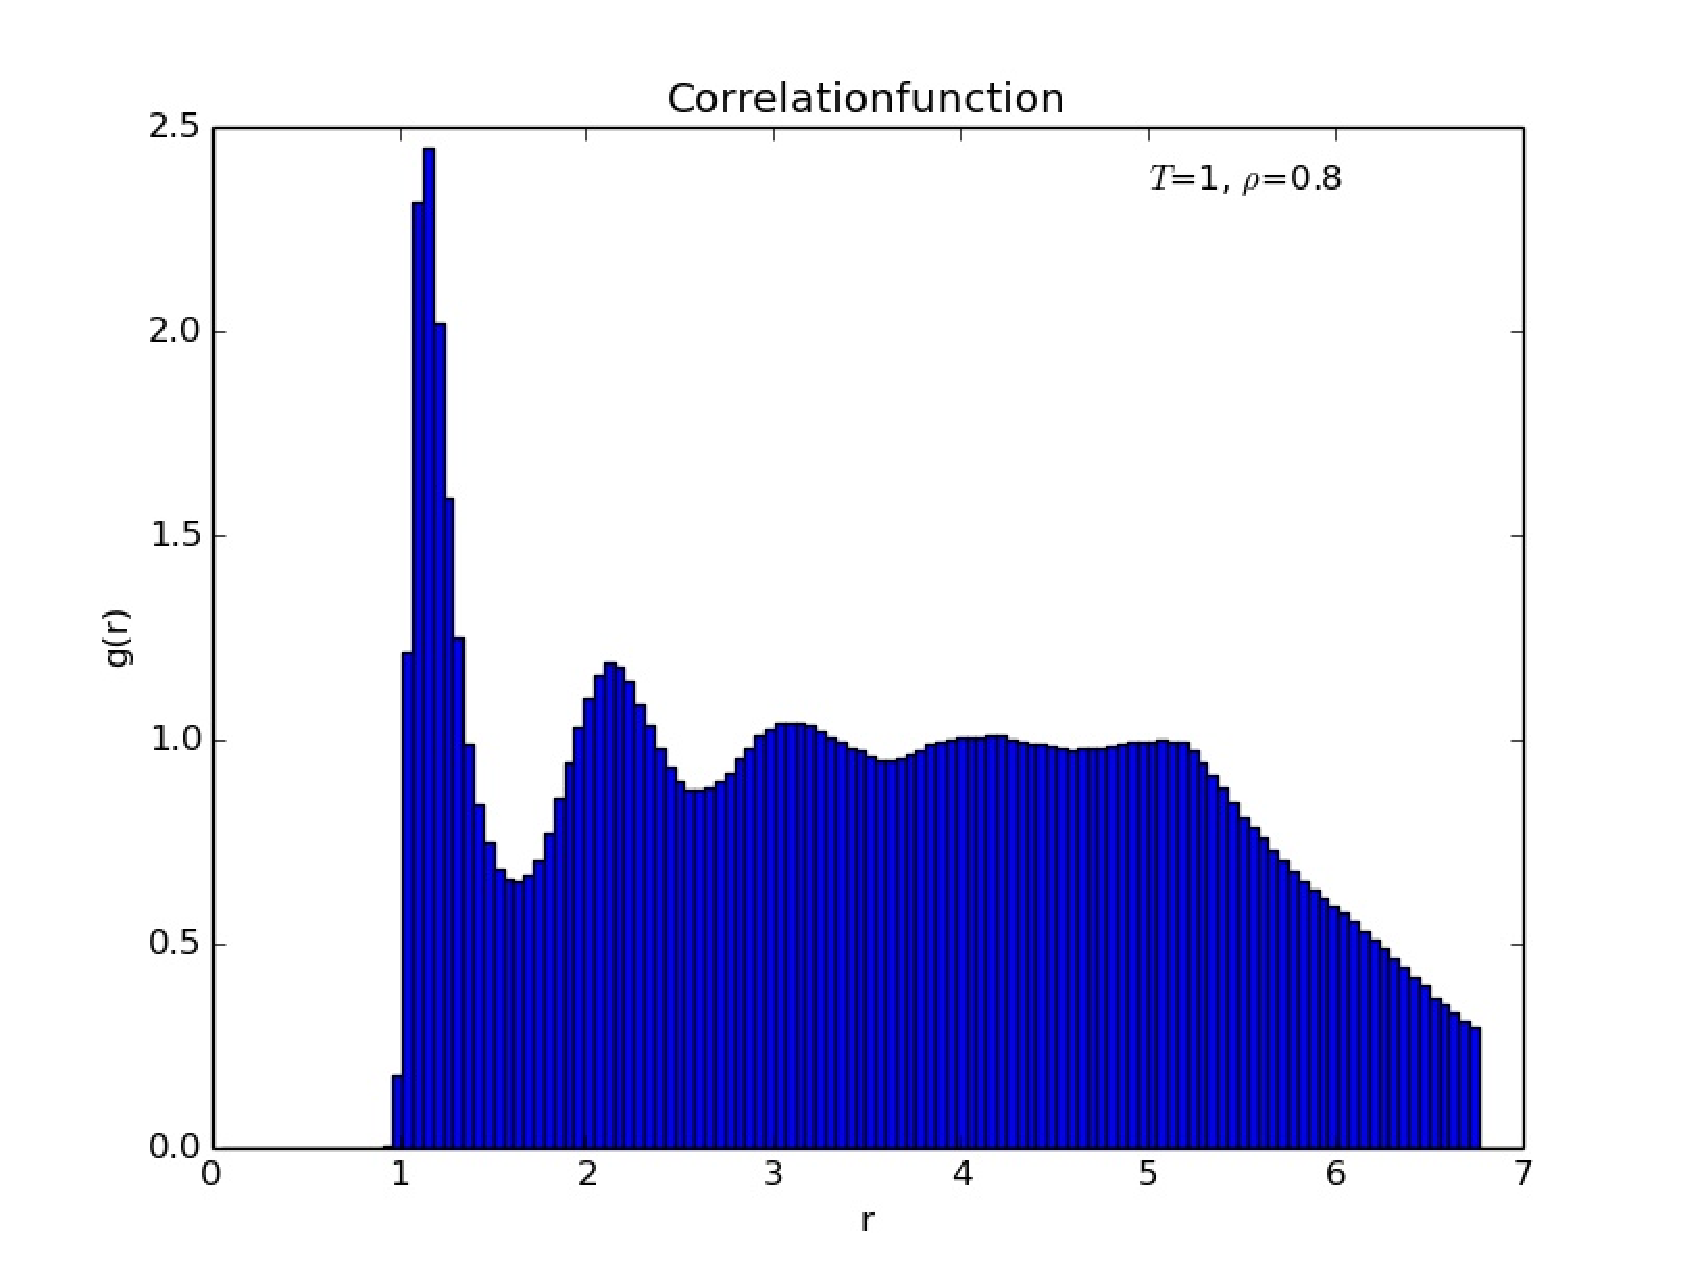
\includegraphics[width=\linewidth]{plots/corfunct1rho08n864lp500.pdf}
\caption{Correlation function for a liquid at $T=1.0$ eV and $\rho=0.5$ $\AA ^{-3}$.  The decaying periodic structure is what we would expect from a liquid - having characteristics between that of a solid and gas.}
\label{corliquid}
\end{center}
\end{figure}

\begin{figure}[H]
\begin{center}
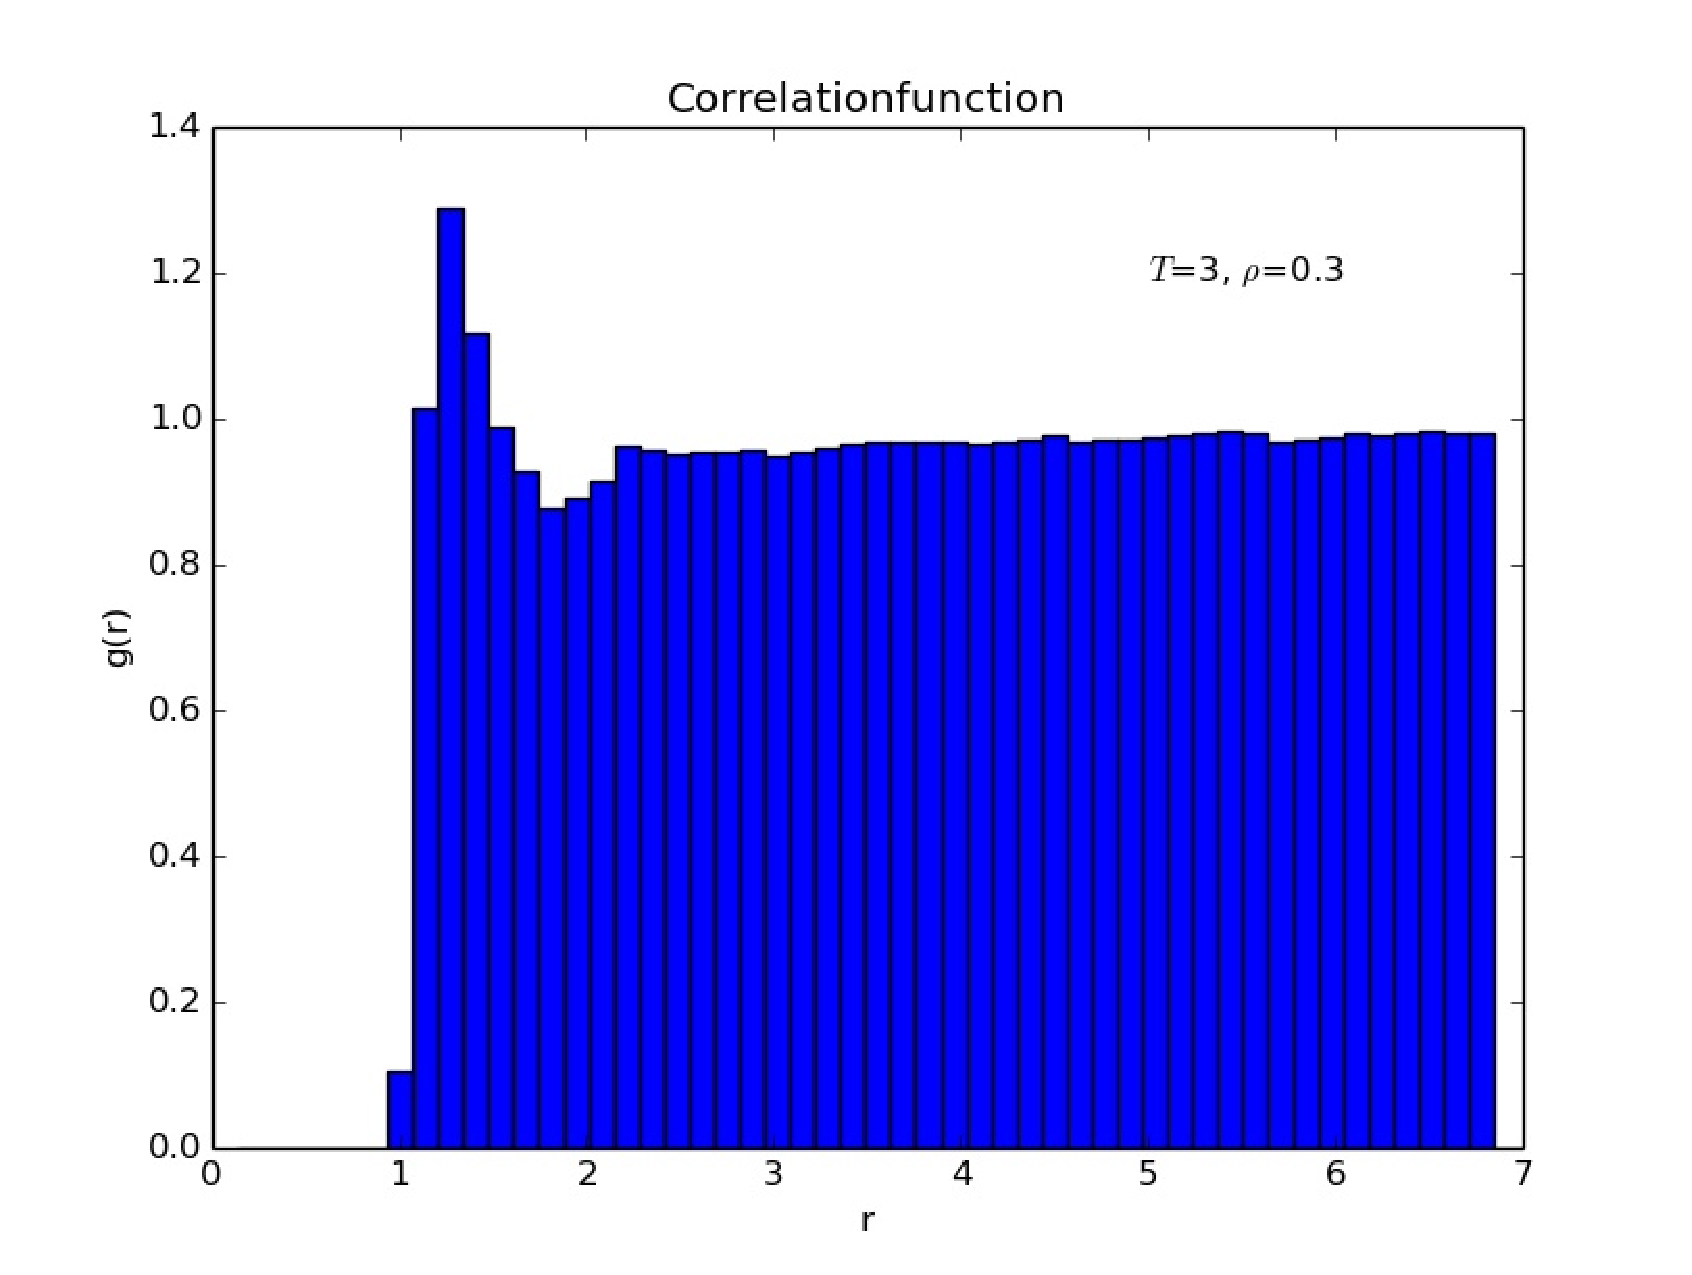
\includegraphics[width=\linewidth]{plots/correlationfunctionT3Rho03x.pdf}
\caption{Correlation function for a gas at $T=3.0$ eV and $\rho = 0.3$ $\AA ^{-3}$.  The exponential decay is the shape that we would expect.}
\label{corgas}
\end{center}
\end{figure}

\subsection{Pressure}

\begin{table*}
\begin{center}
\begin{tabular}{| c | c | c | c | c | c |}
\hline  $T$ [eV] & $\rho$ [$\AA ^{-3}$] & $P$ [eV$\AA ^{-3}$] & $\sigma_{P}$ [eV$\AA ^{-3}$]  & $\sigma_{Pblock}$ [eV$\AA ^{-3}$] & $\sigma_{Pblock}/ \sqrt n$ [eV$\AA ^{-3}$] \\ \hline
  3.0 & 0.5 & 5.4862 & 0.0836 & 0.0089 & 0.0010 \\ \hline
  1.0 & 0.88 & 2.6982 & 0.0171 & 0.0067 & 0.0008 \\ \hline
  0.5 & 1.2 & 1.1105 & 0.0056 & 0.0021 & 0.0002 \\ \hline
\end{tabular}
\label{pressuretab}
\caption{Pressure of a gas, solid, and liquid (top to bottom), at a given temperature $T$ and density $\rho$.  $\sigma _P$ gives the standard deviation of each calculation.  Values of pressure should be quoted as $P \pm \sigma _{Pblock}/\sqrt{N}$.  Numbers can be compared to \cite{thijssen}.}
\end{center}
\end{table*}

The pressure was calculated for the three different values of temperature and density, and is shown in Table 2.  The calculated standard deviation of the the pressure is also given in this table.  \\


\begin{figure}[H]
\begin{center}
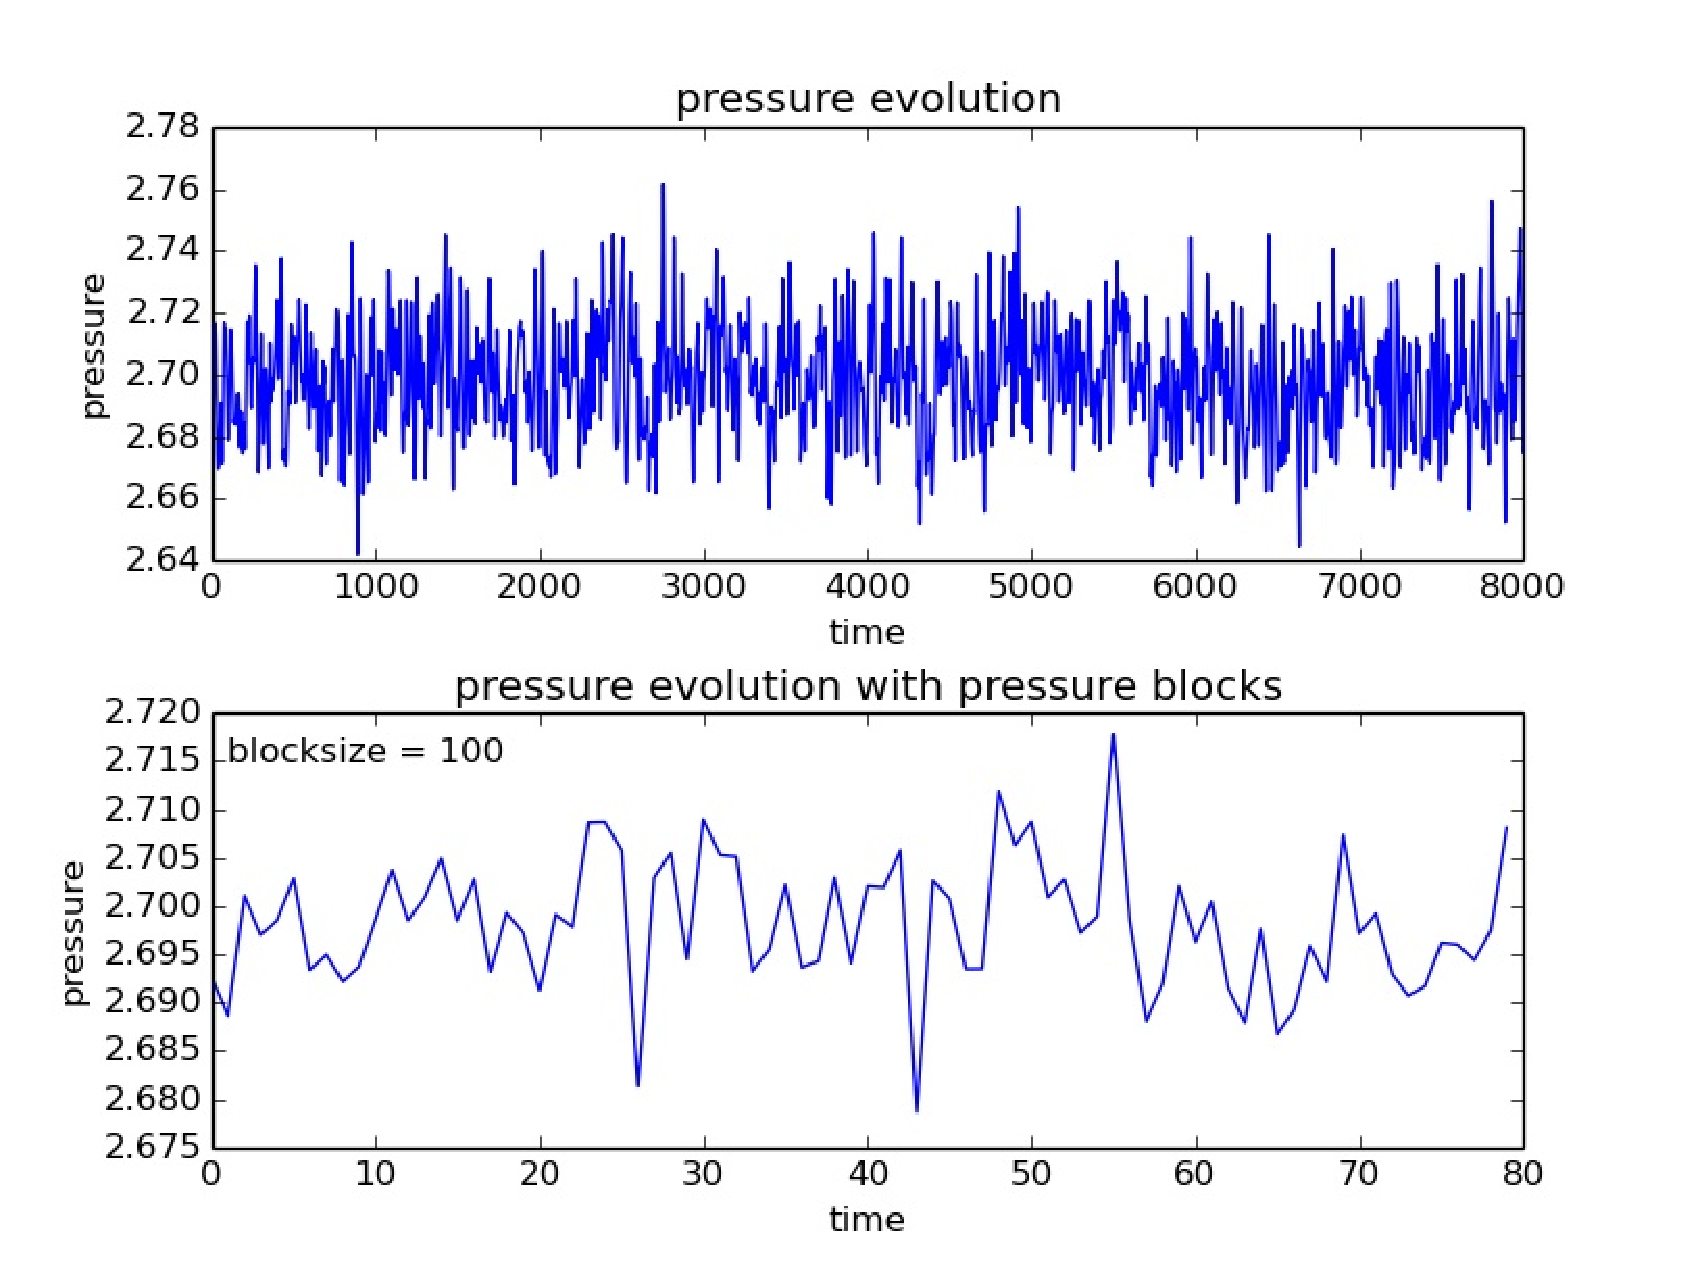
\includegraphics[width=\linewidth]{plots/presn100lp10000T1rho088prt864.pdf}
\caption{Top, pressure calculated for every time step.  Bottom, pressure averaged over every 100 time steps in the top plot. Both graphs for $T = 1$ eV, $\rho = 0.88$ $\AA ^{-3}$}
\label{errex}
\end{center}
\end{figure}

As becomes clear from the upper portion of Figure \ref{errex}, besides strong short time range fluctuations, there is also a longer time range fluctuation.  This can be seen from the fact that for certain time ranges the pressure fluctuates around a higher average than for other time ranges.  In order to measure the long time range fluctuation, we divided the pressure up in blocks of $100$ time steps and took the mean and standard deviation of the block pressure (explained in greater detail in Appendix \ref{errorcalc}).  The standard deviation of the mean of the block pressure is also calculated and can be taken as the error of the pressure.  In the bottom half of Figure \ref{errex} is the block pressure, where one can see that the short time fluctuations are averaged out.\\

The calculated values for the pressure can be compared to values from the literature, \cite{thijssen}, \cite{verlet}. Results from an experiment with the same setup yielded a value of $\frac{P}{\rho} = 2.98$ eV with $\rho = 0.88$ $\AA ^{-3}$, $T = 1$ eV. The value for $P/\rho$ for the same temperature and density that we found was $\frac{P}{\rho} = \frac{2.6982}{0.88} = 3.07 \pm 0.00 $ eV.  The difference appears small but is significant. The reason for this difference is subject to further research.

\section{Conclusion}
\label{conc}

In conclusion, we successfully ran a molecular dynamics simulation of 864 argon atoms.  Beginning in an FCC crystalline lattice with periodic boundary conditions, we simulated contact with thermostats of target temperatures $T=3.0$ eV, $T=1.0$ eV, and $T=0.5$ eV.  From there, we calculated calculated properties of a gas at $T=0.49983 \pm 0.000111$ eV, $\rho=0.3$ $\AA ^{-3}$ with $P=5.4862 \pm 0.0010 $ eV$\AA^{-3}$, a liquid at $T= 1.01501 \pm 0.000203$ eV, $\rho =0.8$ $\AA ^{-3}$ with $P=2.6982 \pm 0.0008$ eV$\AA^{-3}$, and a solid with $T=2.975473 \pm 0.000365$  eV, $\rho=1.2$ $\AA ^{-3}$ at $P=1.1105 \pm 0.0002 $ eV$\AA^{-3}$.  With the exception of some of the pressure values, our current calculations agree with those of previous work under similar conditions.  \\

Further work can still be done.  There are other interesting thermodynamical quantities that can be calculated for this system, such as the specific heat, chemical potential, and free energy.  It would also be interesting to change the initial conditions of the system.  Instead of periodic boundary conditions, put the system in a physical box and see how the interactions with the wall change the observables.  Also, a different crystalline structure (such as HPC) could be used as the initial configuration.  This would allow us to see whether the system did rearrange itself into the true FCC ground state of argon. 

\appendix 

\section{Error Calculations}
\label{errorcalc}

Like experimental measurements, numerical calculations should include error bars.  Just as in an experiment where we would ideally take many measurements and calculate an error based on their standard deviations from the mean, we can use the same concept to put error bars on our calculated values.  There are many ways that these uncertainties can be calculated, but in this paper, we will be using a result of the ergodic theorem \cite{Birkhoff}, that the spatial average is equal to the time average.  \\

There are several ways that we can calculate a time average for our calculation.  Perhaps, the most obvious one is to run the calculation several times to generate a mean and a standard deviation.  However, this process is lengthy and can be heavily dependent on the seed of the random number generator used in initializing positions and velocities the particles.  \\



It is, therefore, much better to run one simulation and average over many blocks of time.  In each simulation, after a long enough period of time, the quantity of interest will settle on some mean value with every time step oscillating around this value, as show in Figure \ref{errex}.  While each value depends on the previous value, averaging over a large enough number of time steps will produce a value independent of the previous block of time steps.  For each of these blocks, 100 time steps, an average is calculated (this is equivalent to having many measurements from an experiment), and then from each of these numerical measurements, we can calculate an average value for our simulation and an error for that value.  The average value is defined as 

\begin{equation}
\bar{C} = \frac{1}{N}\sum \limits _{i=1}^N C_i 
\end{equation}

\noindent and the error is calculated from 

\begin{equation}
\delta ^2 = \frac{1}{N}\sum \limits _{i=1}^N (C_i - \bar{C})^2
\end{equation}

\noindent where $\delta$ is the error on a given quantity, $N$ is the number of time-step blocks, and $C_i$ is the quantity value for each time step block.  Throughout this report, $\delta$ is denoted as $\sigma /\sqrt{N}$.  \\

This process ensures that we include fluctuations in the quantities that we report, as well as account for a decreasing error as the number of measurements increases.  \\

\end{multicols}

\bibliography{MolDynBib}

%\begin{thebibliography}{99}

%\bibitem{deGroot}
  %B. de Groot,
  %Computational Biomolecular Dynamics Group, Max Planck lnstitute for Biophysical Chemistry. %Retrieved from http://www3.mpibpc.mpg.de/groups/de_groot/
  
%\bibitem{thijssen}
 % Thijssen, J.M.(2007). Computational Physics. Cambridge, Cambridge University Press.
%\end{thebibliography}

\end{document}
